%%%%%%%%%%%%%%%%%%%%%%%%%%%%%%%%%%%%%%%%%%%%%%%%%%%%%%%%%%%%
%                          OPTIONS
%%%%%%%%%%%%%%%%%%%%%%%%%%%%%%%%%%%%%%%%%%%%%%%%%%%%%%%%%%%%
\documentclass[a0,50pt]{a0poster}
\usepackage[absolute]{textpos}
\usepackage{tikz}
\usepackage{tcolorbox}

\usepackage[utf8]{inputenc}
\usepackage[L7x]{fontenc}
\usepackage[lithuanian]{babel}

\setlength{\paperheight}{119cm}
\setlength{\paperwidth}{84cm}
\TPGrid[0.5cm,1cm]{119}{84}
\setlength{\TPHorizModule}{1cm}
\setlength{\TPVertModule}{1cm}

\graphicspath{{./figures/}}

% Font
\renewcommand{\familydefault}{\sfdefault}
\usepackage{lmodern} 
\usepackage{xcolor}
\definecolor{fontMain}{HTML}{480025}
\definecolor{fontMain2}{HTML}{002548}
\definecolor{boxfill}{HTML}{f5f2f4}

\let\Textsize\normalsize
\def\Title#1{\noindent{\textbf{\veryHuge\color{fontMain} #1}}}
\def\Authors#1{\noindent{\Large\color{fontMain2} #1}\bigskip}
\def\SectionTitle#1{\noindent{\huge\color{fontMain2} #1}}
\def\CoverTitle#1{\noindent{\textbf{\VERYHuge\color{white} #1}}}


\tikzset{
    mybackground/.style={execute at end picture={
        \begin{scope}
              \draw[fontMain,line width=0.1cm,fill=white,rounded corners=5ex](
                    current bounding box.south west) rectangle (current bounding box.north east);
        \end{scope}
    }},
}


\begin{document}

    % TOP-Seq cover
    \begin{textblock}{0}(0,0)
            \includegraphics[scale=0.9]{meta_Cover}
    \end{textblock}

    \begin{textblock}{20}(5.2,2)
        \CoverTitle{TOP-seq}
    \end{textblock}
    \begin{textblock}{20}(5.2,6.5)
        \CoverTitle{Estimation}
    \end{textblock}


    \begin{textblock}{1}(4.2,15)
        \footnotesize\textit{PG}
    \end{textblock}
    \begin{textblock}{1}(10.6,18.8)
        \footnotesize\textit{MS}
    \end{textblock}
    \begin{textblock}{1}(18.2,23)
        \footnotesize\textit{JG}
    \end{textblock}


    % Logo
    \begin{textblock}{0}(71,0)
            
\includegraphics[scale=1]{meta_logo_VU}
    \end{textblock}
    \begin{textblock}{0}(80,1.1)
            
\includegraphics[scale=1.3]{meta_logo_BTI}
    \end{textblock}

    % Authors
    \begin{textblock}{50}(30,1)
        \begin{center}
            \Authors{\underline{Povilas Gibas}, Mantas Šarauskas and Juozas Gordevičius}
        \end{center}
    \end{textblock}
    \begin{textblock}{50}(30,2.5)
        \begin{center}
            \Authors{\textit{Institute of Biotechnology, Life Sciences Centre, \\Vilnius university, Lithuania}}
        \end{center}
    \end{textblock}

    % Title
    \begin{textblock}{50}(30,6.5)
        \begin{center}
            \Title{Estimation of DNA modification using artificial neural networks from TOP-seq data augmented with genomic context information}
        \end{center}
    \end{textblock}

    \begin{textblock}{50}(28,17.7)
        \Large
        \begin{itemize}
            \item DNA modifications have been implicated in aetiology of complex disease
            \item Epigenome-wide association studies are limited either by resolution or by the cost of existing technologies
            \item We leverage novel TOP-seq\textsuperscript{1} unmethylome profiling technology that yields 3.9x coverage of 7.3M genomic CG sites with 57M reads
            \item Our computational strategy leads to r=0.77 genome-wide correlation of TOP-seq\textsuperscript{1} with whole genome bisulfite seq (WGBS) and r=0.9 in gene regions
        \end{itemize}
    \end{textblock}

    \begin{textblock}{18}(0,31)
        \begin{tikzpicture}[mybackground={}]
            \node[minimum width=24.7cm,minimum height=77cm]{};
        \end{tikzpicture}
    \end{textblock}
    \begin{textblock}{25}(0.55,31.8)
        \begin{center}
            \SectionTitle{TOP-seq\textsuperscript{1}: direct readout of individual unmethylated CG sites}
        \end{center}
    \end{textblock}
    \begin{textblock}{0}(0.8,39)
            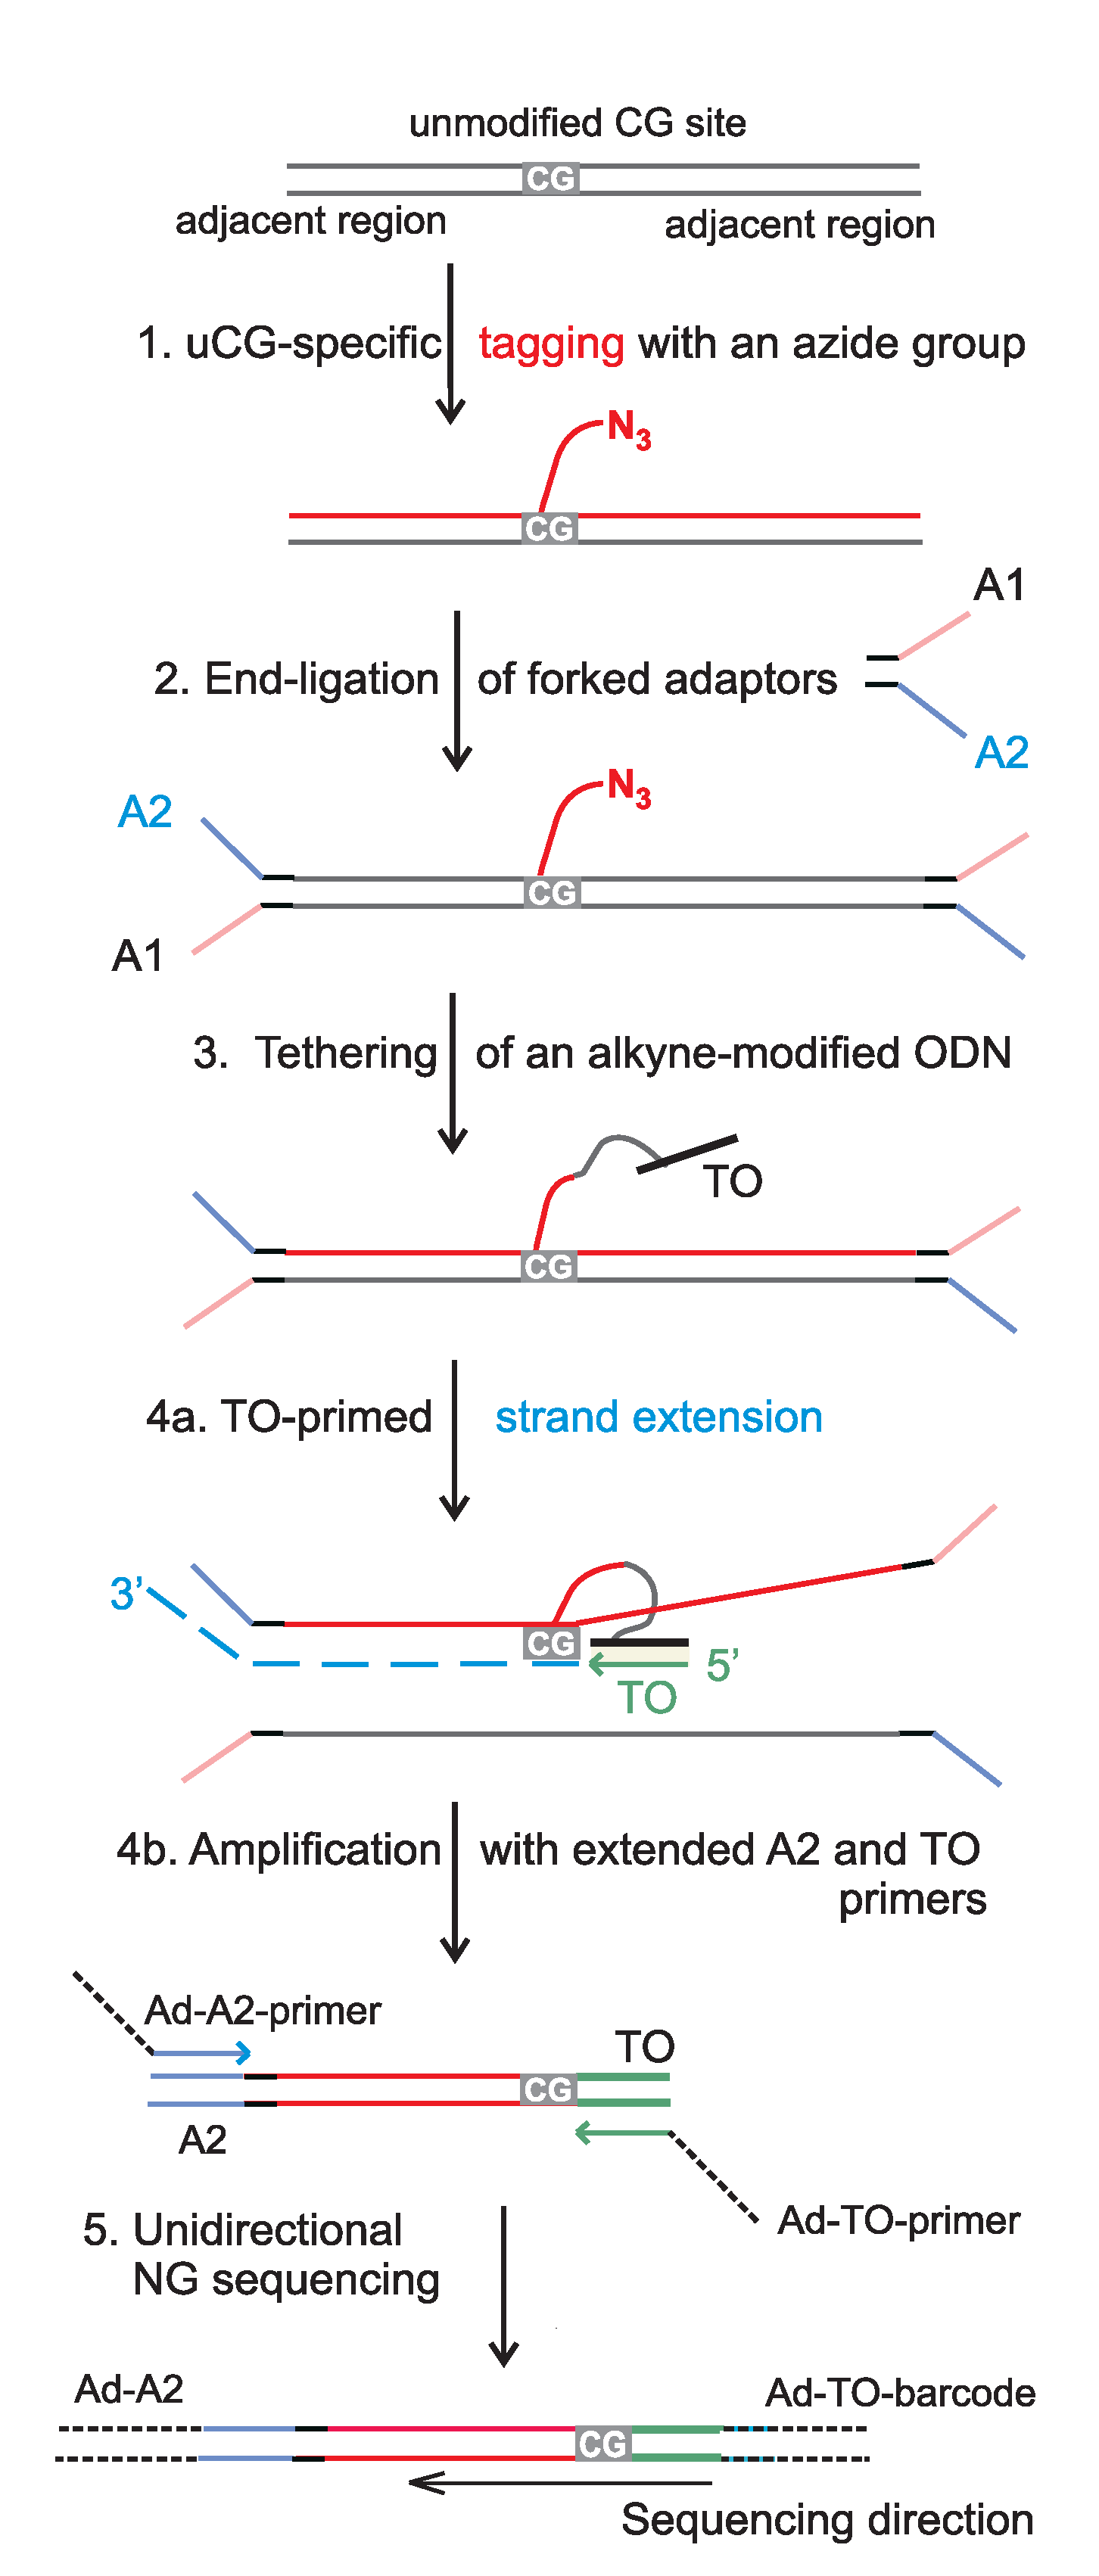
\includegraphics[scale=0.9]{TOP-Seq_Scheme}
    \end{textblock}
    \begin{textblock}{20}(3,95)
        \Large98\% of reads start within 2bp of CG
    \end{textblock}
    \begin{textblock}{0}(4,97)
        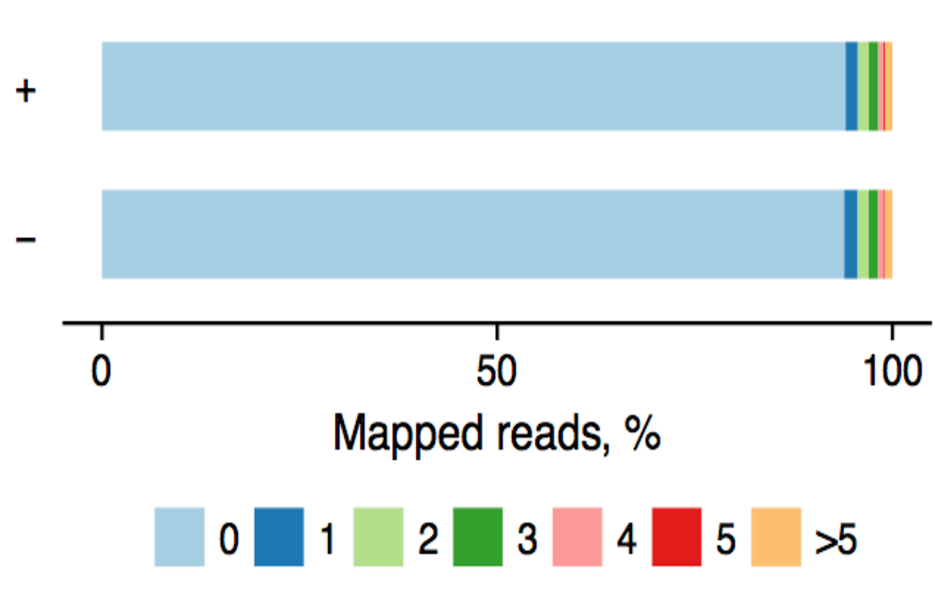
\includegraphics{TOP-Seq_distance}
    \end{textblock}



    \begin{textblock}{50}(26.8,31)
        \begin{tikzpicture}[mybackground={}]
            \node[minimum width=54.6cm,minimum height=38cm]{};
        \end{tikzpicture}
    \end{textblock}

    \begin{textblock}{25}(29,32.4)
            \SectionTitle{Method}
    \end{textblock}

    \begin{textblock}{25}(29,36)
        \Large
        \begin{itemize}
            \item IMR90 cell line sequenced using TOP-seq\textsuperscript{1} used for prediction
            \item IMR90 WGBS data (Lister et al., Ziller et al.) for training and evaluation
            \item A multi-layer perceptron regressor with 2 hidden layers (44 and 22 nodes respectively) was trained using stochastic gradient descent on chromosome 20 (2.5\% CG sites in the genome)
        \end{itemize}
    \end{textblock}

    \begin{textblock}{25}(56,32.4)
        \SectionTitle{Input features}
    \end{textblock}

    \begin{textblock}{25}(56,36)
        \Large
        \begin{itemize}
            \item TOP-\textsuperscript{1} coverage and u-density for each CG in the genome
            \item Genome element information (gene, CpG island, repeat etc. status)
            \item Sequence context information around each CG in 50bp window (CG\%, GC\%, C ratio, mappability, GERP score)
            \item Nucleotide sequence around CG in 3bp window
        \end{itemize}
    \end{textblock}

    % \begin{textblock}{0}(29,54)
    %     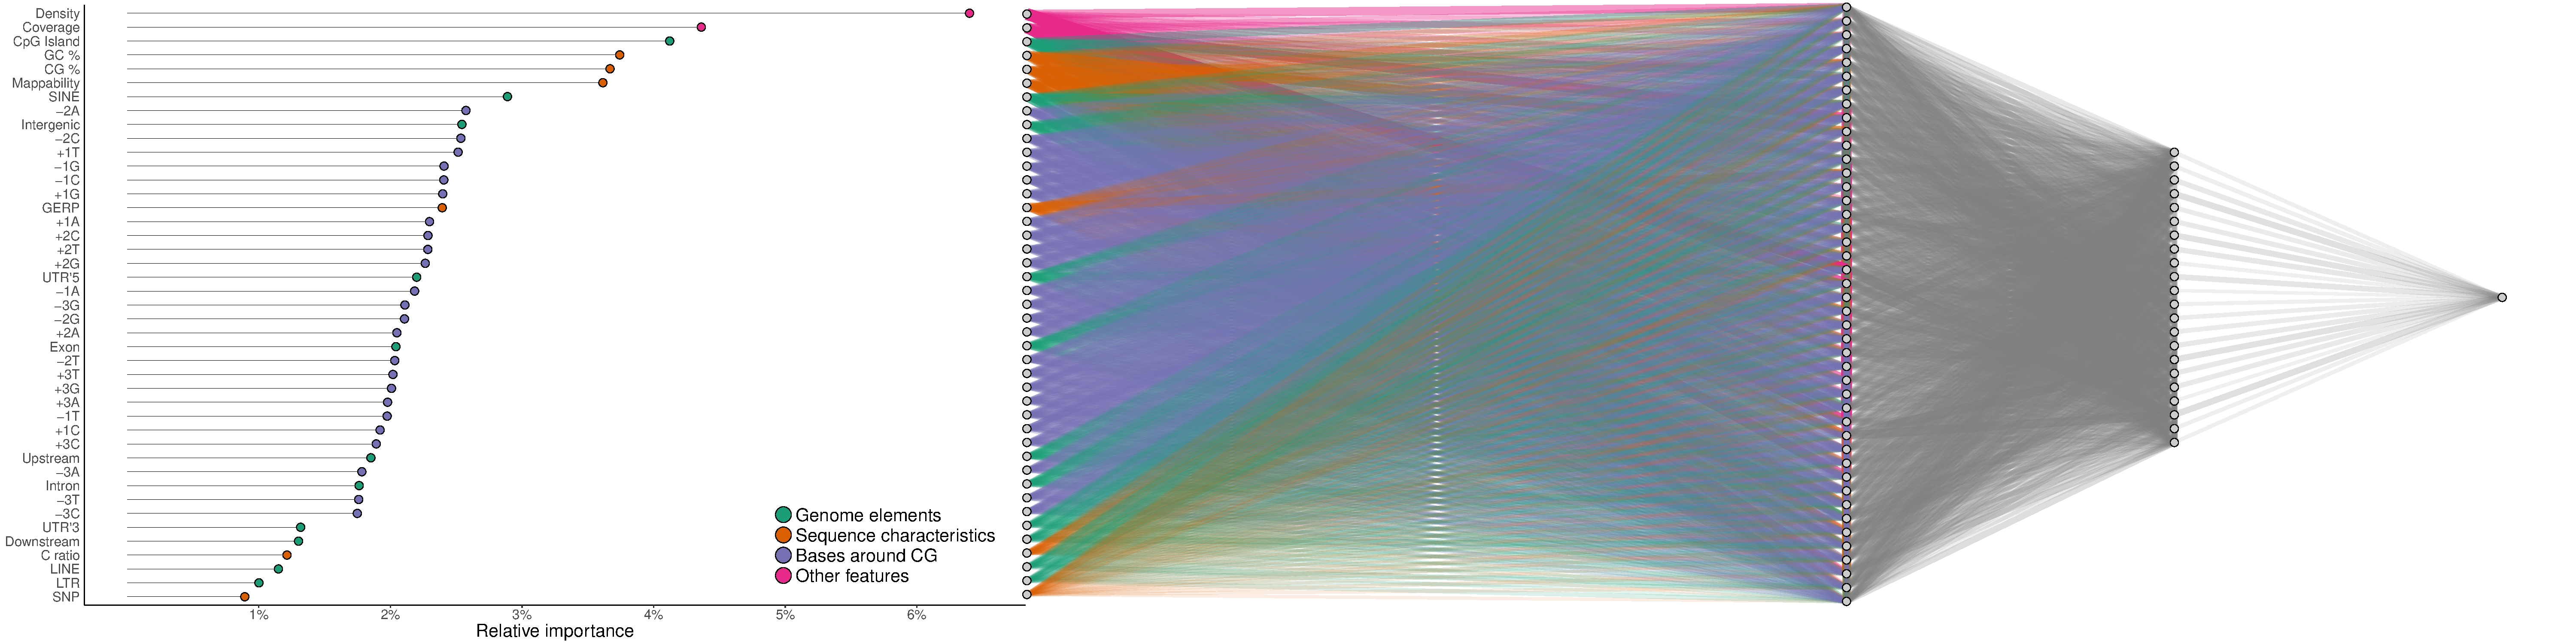
\includegraphics[scale=0.51]{figure_1}
    % \end{textblock}

    \begin{textblock}{50}(26.8,72)
        \begin{tikzpicture}[mybackground={}]
            \node[minimum width=54.6cm,minimum height=44.9cm]{};
        \end{tikzpicture}
    \end{textblock}

    \begin{textblock}{25}(29,73.4)
        \SectionTitle{Results}
    \end{textblock}

    \begin{textblock}{25}(29,77)
        \Large
        \begin{itemize}
            \item Correlation between WGBS and predicted values in protein coding genes (n = 18.5k):\\
            with WGBS 1 (used for training) Pearson r = 0.9, with WGBS 2 (used for evaluation) Pearson r = 0.8
        \end{itemize}
    \end{textblock}

    \begin{textblock}{25}(56,77)
        \Large
        \begin{itemize}
            \item Applying regressor model on CpG islands with simulated differential coverage (observed average coverage was scaled by a given factor) yields a corresponding change in predicted values.
        \end{itemize}
    \end{textblock}

    \begin{textblock}{25}(56,99)
        \Large
        \begin{itemize}
            \item Correlation between WGBS 1 and predicted values in different chromosomes. For a subset of random CG (20K) scatter plots between the two measurements are shown on the left.
        \end{itemize}
    \end{textblock}

    % \begin{textblock}{0}(29,86)
    %     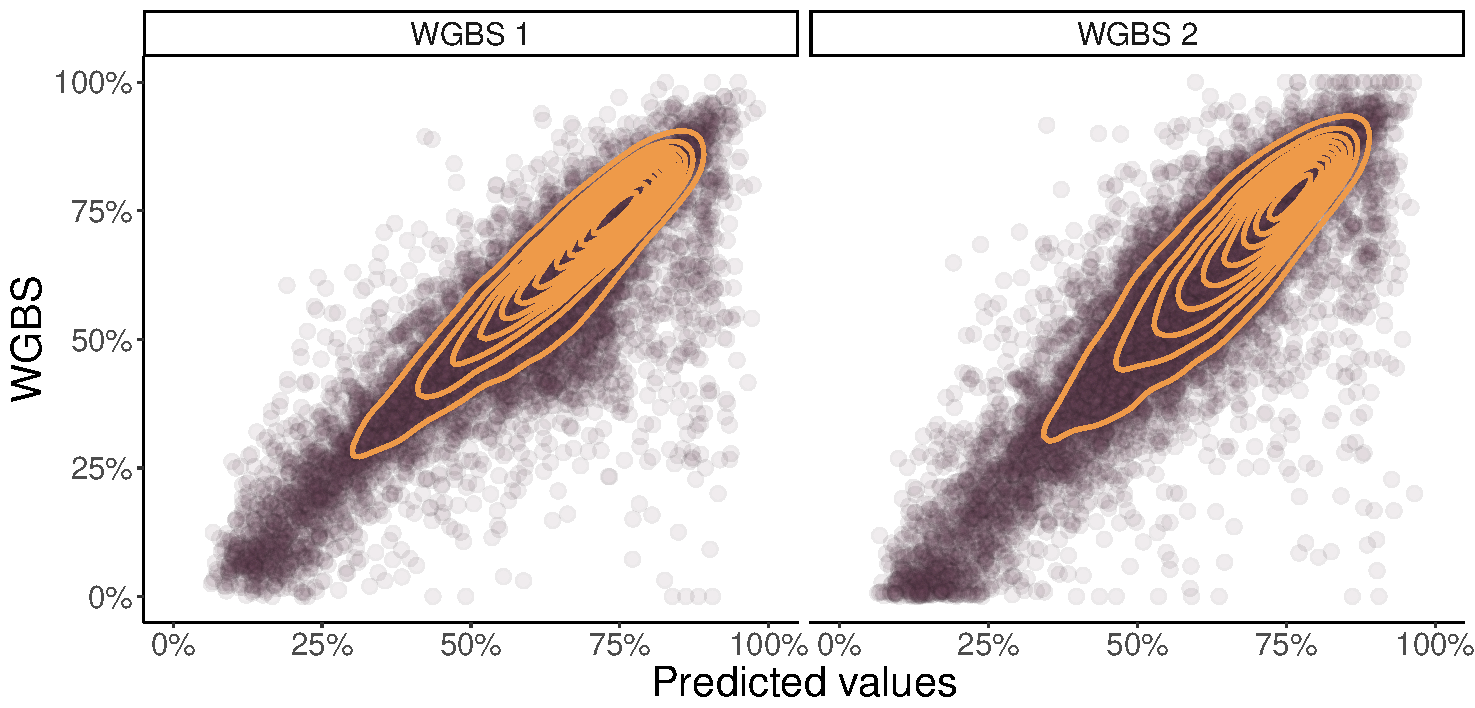
\includegraphics{figure_2}
    % \end{textblock}
    % \begin{textblock}{0}(29,98)
    %     \includegraphics{figure_3}
    % \end{textblock}
    % \begin{textblock}{0}(56,84)
    %     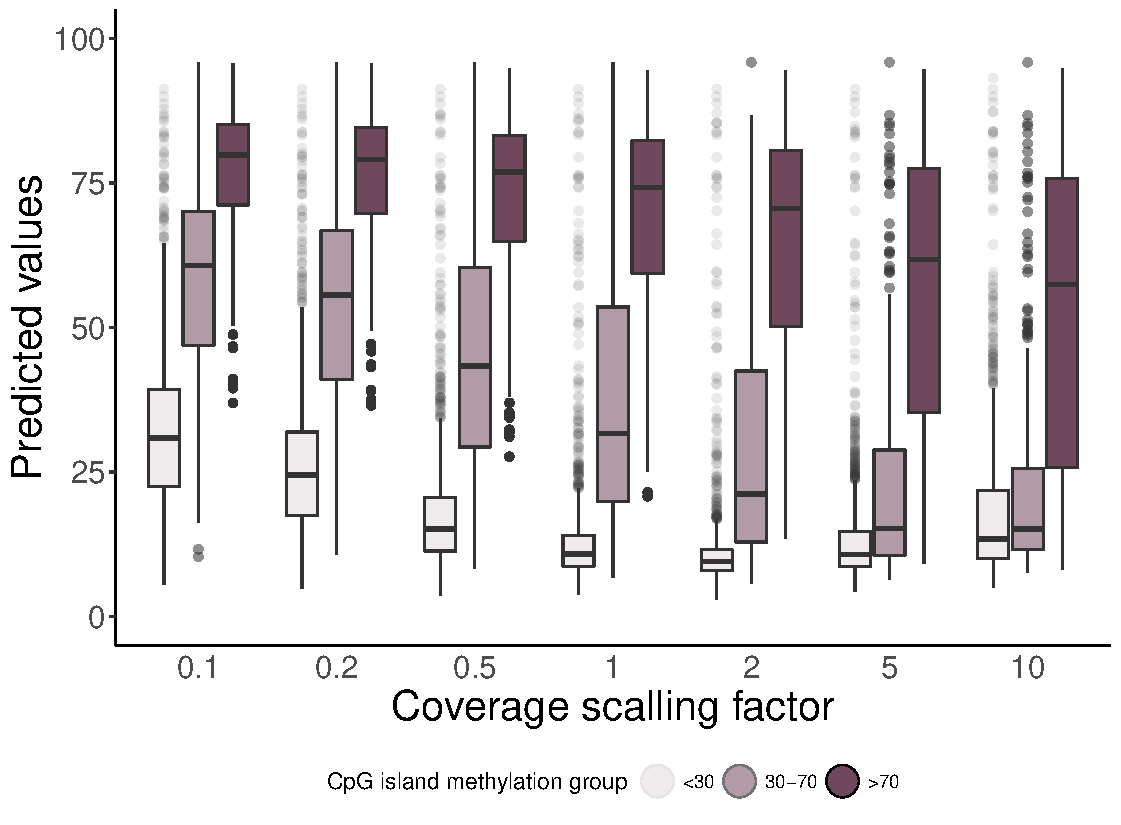
\includegraphics{figure_4}
    % \end{textblock}
    % \begin{textblock}{0}(56,106)
    %     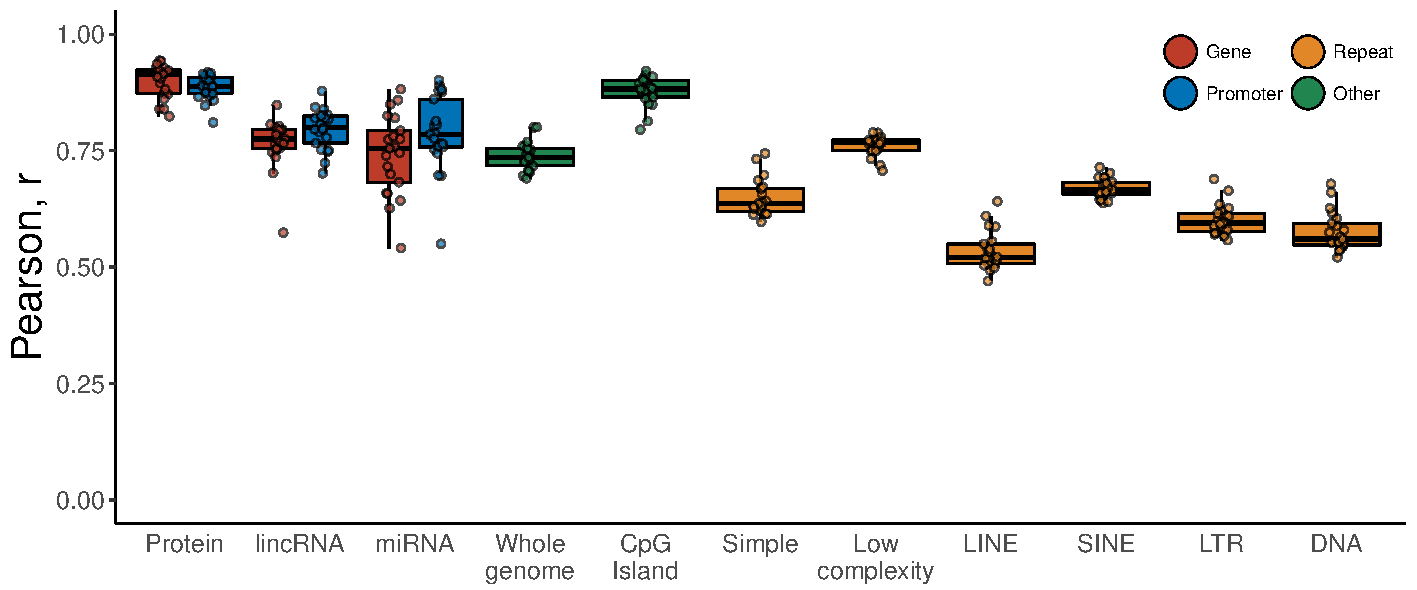
\includegraphics{figure_5}
    % \end{textblock}

    % References
    \begin{textblock}{22}(2,109)
        \renewcommand{\section}[2]{}
        \begin{thebibliography}{}
            \bibitem{Stasevskij}
                Staševskij et al.
                \newblock Tethered Oligonucleotide-Primed Sequencing, TOP-Seq: A High-Resolution Economical Approach for DNA Epigenome Profiling.
                \newblock {\em Mol Cell}, 65:554--564, 2017.
            \bibitem{Lister}
                Lister et al.
                \newblock Human DNA methylomes at base resolution show widespread epigenomic differences.
                \newblock {\em Nature}, 462:313--322, 2009.
            \bibitem{Ziller}
                Ziller et al.
                \newblock Charting a dynamic DNA methylation landscape of the human genome.
                \newblock {\em Nature}, 500:477--481, 2013.

        \end{thebibliography}
    \end{textblock}
\end{document}